\chapter{High-pass and low-pass filters}
The main purpose of filters is to sort out unwanted frequencies from different wave-types. Filters are often used on sound files, to control the bass or the high pitch noises. There are different kinds of filters that can sort out unwanted frequencies. In this section the focus is on high and low-pass filters.
\section{Definitions}
In this section the most central terms concerning high-pass and low-pass filters will be defined. The definitions are essential when understanding the most important derivations in the next section \ref{Derivations}.
\subsection{bla bla}
In the experiment earlier described a DC input was used. In the case of high and low pass filters an AC input will be applied. The voltage in this case can be written as a wave function:
\begin{align}
 v(t)=A\sin(\omega t+\theta)
 \end{align} 
Where $A$ is the amplitude, $\omega=2\pi f$ and $\theta$ the phase shift. 
\\
This sinus function can be rewritten as a complex exponential function.
\begin{align*}
v(t)=Ae^{i\omega t}
\end{align*}
\subsection{Low-pass filters}
The purpose of a low-pass filter is to filter out unwanted high frequencies. Listening to a such tone brings out the bass and sorts out higher pitches. The low-pass filter is in other words allowing frequencies from $0Hz$ to a chosen cut-off value. \\
The difference between a high-pass filter and a low-pass can be illustrated using a circuit diagram:
\begin{figure}[H]
	\begin{center}
\begin{circuitikz}[american voltages]
\draw (0,0)
to[sqV, sqV=$V_{AC}$] (0,2)
to (6,2)
to[short, -] (4,2)
to[C=$C$] (4,0)
to (6,0)
to (4,0)
to [resistor, R=$R$] (0,0);
\draw [>=latex', <->] (6,1.75) -- node[anchor=west] {$V_{output}$} (6,0.25);
\end{circuitikz}
\end{center}

	\caption{Circuit diagram of a low-pass filter.} \label{lp:diagram}
\end{figure} 
In the illustration above the voltage output is measured across the capacitor, which decreases the high frequencies and leaves the low frequencies unchanged.  
\subsection{High-pass filters}
High-pass filters are in many ways similar to the low-pass filters. High-pass filters can be used with the purpose of decreasing low frequencies and leave the high frequencies unchanged. Listening to a such tone would cut off some of the base and leave the lower tones unchanged. \\
The circuit diagram for the high-pass filter is the same as the low-pass filter, but the voltage output is measured around the resistor ($R$) instead of the capacitor ($C$). This is commonly shown by switching around the two, from the previous figure \ref{lp:diagram}:
\begin{figure}[H]
	\begin{center}
\begin{circuitikz}[american voltages]
\draw (0,0)
to[sV, sV=$V_{AC}$] (0,2)
to (6,2)
to[short, -] (4,2)
to[resistor, R=$R$] (4,0)
to (6,0)
to (4,0)
to [C=$C$] (0,0);
\draw [>=latex', <->] (6,1.75) -- node[anchor=west] {$V_{output}$} (6,0.25);
\end{circuitikz}
\end{center}

	\caption{Circuit diagram of a high-pass filter.}
	\label{hp:diagram}
\end{figure} 
Measuring across the resistor decreases the low frequencies and leaves the high frequencies unchanged. 
\subsection{Cut-off Frequencies}
For low-pass \\
This cut-off value can be calculated using the following equation:
\begin{align*}
f_{cutoff}=\dfrac{1}{2 \pi RC}
\end{align*}
This cut-off value describes a point on the bode plot graph, where the amplitude is decreased by $29.3\%$ and the output is decreased by $3dB$. The cut-off point is also the point, where the filtering starts getting efficient. This can be expressed using a bode plot, with the frequency on the $x-axis$ and the decibel on the $y-axis$.\\
For high-pass: \\
The high-pass filters uses the same $f_{cutoff}$ formula as the low-pass filter.

\subsection{Bode Plots}
Low-pass: \\
The $x-axis$ is a logarithmic axis, where the output is decreased by 20 decibel per decade after the cut-off point. \\
The output wave before the cut-off point will stay almost unchanged, and after the cut-off point, the amplitude is decreasing and approaching a graph that looks like a DC current. \\
High-pass: \\
When plotting the graph for the high-pass filter, the bode plot is going to be the opposite of the low-pass filters'. The graph starts in minus decibel and is approaching zero. Until it reaches the cut-off point, the graph is increasing with 20 decibel per decade. When reaching the cut-off point, the graph is 3 decibel short from reaching zero. Furthermore, $70.7\% (100\%-29.3\%)$ of the amplitude is cut off at the point $f_{cutoff}$.
\subsection{The imaginary Angular Frequency}
- Describe
\section{Derivations} \label{Derivations}
In section the most essential terms used in the experiment \ref{experiment} is derived. 
\subsection{Transfer Function for Low-Pass Filters}
From the transient analysis in EQBLAH this equation is derived:
\begin{align} \label{eq:dV_C}
\dfrac{dv_C(t)}{dt}=-v_R(t)\dfrac{1}{RC}
\end{align}
Here $-v_{R}(t)$ can be rewritten as 
\begin{align} \label{eq:vr}
-v_{R}(t) = v_{c}(t) + v_{input}, 
\end{align}
since $-v_{input}(t)+v_{R}(t)-V_{C}(t)=0$. These are all functions of time. It is all inserted on \eqref{eq:dV_C}:
\begin{align} 
\dfrac{dv_C(t)}{dt}=\Big(v_C(t) + v_{input}(t)\Big)\dfrac{1}{RC}
\end{align}
$\omega$ is defined as $\omega=\dfrac{1}{RC}$:
\begin{align}
\dfrac{dv_C(t)}{dt}=\Big(v_C(t)+v_{input}(t)\Big)\omega
\end{align}
Now $\omega$ is multiplied in the parenthesis and $v_{input}(t)$ is isolated:
\begin{align}
v_{input}(t)\omega=v_C(t)\omega+\dfrac{dv_C(t)}{dt}
\end{align}
The differential equation can now be solved using Laplace transform:
\begin{align}\label{eq:laplace:low}
\mathcal{L}\Big\{v_{input}(t)\Big\}\omega=\mathcal{L}\Big\{v_C(t)\Big\}\omega+\mathcal{L}\bigg\{\dfrac{dv_C}{dt}\bigg\}
\end{align}
According to \Cref{theorem:laplace_diff} the Laplace transform of \eqref{eq:laplace:low} yields the following equation:
\begin{align}
V_{input}(s)\omega=V_{C}(s)\omega-v_{C}(0)+V_{C}(s)s
\end{align} 
$v_{C}$ is now factorised, and the voltage across the capacitor at time zero is zero, which can be derived from equation \eqref{V_up}:
\begin{align}
V_{input}(s)\omega=V_{C}(s)(\omega+s)
\end{align} 
The functions of voltage are isolated:
\begin{align}
\dfrac{\omega}{\omega+s} = \dfrac{V_{C}(s)}{V_{input}(s)}
\end{align} 
As stated in REF then $s=i \omega_f$. Furthermore, the expression $\dfrac{V_{C}(s)}{V_{input}(s)}$ is defined as the transfer function for low-pass filters, $H_{L}(s)$. Since $s$ is redefined the $H_{L}(s)=H_{L}(i \omega_f)$:
\begin{align}
H_{L}(s) = \dfrac{\omega}{\omega+i \omega_f} 
\end{align}
$\omega = \dfrac{1}{RC}$ is inserted and the whole expression is multiplied by $\dfrac{RC}{RC}$:
\begin{align}
H_{L}(s) = \dfrac{RC}{RC} \cdot \dfrac{\dfrac{1}{RC}}{\dfrac{1}{RC}+i \omega_f} 
\end{align}
This can be simplified:
\begin{align}
H_{L}(s) =  \dfrac{1}{1+RC \cdot i \omega_f} 
\end{align}
Now the length of the both sides is calculated:
\begin{align}
\left|H_{L}(s) \right| =  \left|\dfrac{1}{1+RC \cdot i \omega_f} \right| 
\end{align}
This can be rewritten as:
\begin{align}
\left|H_{L}(s) \right| =  \dfrac{1}{\sqrt{1+(RC \cdot i \omega_f)^2}}
\end{align}
\subsection{Transfer Function for High-Pass Filters}
\begin{align}
\dfrac{dv_{c}(t)}{dt} = -v_{R}(t) \cdot \dfrac{1}{RC}
\end{align}
First both sides are multiplied by $-RC$:
\begin{align}
-RC \cdot \dfrac{dv_{c}(t)}{dt} = v_{R}(t)
\end{align}
Since it is now a high-pass filter (and a different circuit), kirchhoff's voltage law has to be rewritten from equation \eqref{eq:vr}, and is now $v_{C}(t)=v_{R}(t)-v_{input}(t)$. Both sides of this expression is now differentiated, and can be inserted on the left side as follows:
\begin{align*}
-RC \cdot \left(\dfrac{dv_{R}(t)}{dt} - \dfrac{dv_{input}(t)}{dt} \right) = v_{R}(t)
\end{align*}
Now the Laplace transform of both sides can be made. Note that $RC$ is a constant and can be moved outside the transform per definition \ref{constant}:
\begin{align*}
-RC \mathcal{L} \left\{\dfrac{dv_{R}(t)}{dt} \right\} + RC \mathcal{L} \left\{ \dfrac{dv_{input}(t)}{dt} \right\} = \mathcal{L} \left\{v_{R}(t) \right\}
\end{align*}
The values can be found from the table \ref{lptable} in the previous chapter:
\begin{align*}
-RCsV_{R}(s)-v_{R}(0) + RCsV_{input}(s)-v_{input}(0) = V_{R}(s)
\end{align*}
There is here an assumption that there are no phase shift and $v_{R}(0)$ and $v_{input}(0)$ are both equal zero:
\begin{align*}
-RCsV_{R}(s) + RCsV_{input}(s) = V_{R}(s)
\end{align*}
Now $V_{input}(s)$ is isolated:
\begin{align*}
RCsV_{input}(s) = V_{R}(s) + RCsV_{R}(s)
\end{align*}
$V_{R}(s)$ is factorised:
\begin{align*}
RCsV_{input}(s) = V_{R}(s) \cdot (1 + RCs)
\end{align*}
The voltage functions are isolated:
\begin{align} \label{hp:visolated}
\dfrac{RCs}{1 + RCs} = \dfrac{V_{R}(s)}{V_{input}(s)}
\end{align}
The expression $\dfrac{V_{R}(s)}{V_{input}(s)}$ can be described as the transfer function of high-pass filters, $H_{H}(s)$. As stated in REF then $s=i \omega_f$. Therefore $H_{H}(s)=H_{H}(i \omega_f)$. The equation \eqref{hp:visolated} can be rewritten:
\begin{align*}
H_{H}(i \omega_f) = \dfrac{RCi \omega_f}{1 + RCi \omega_f}
\end{align*}
The length of both sides can be calculated:
\begin{align*}
\left|H_{H}(i \omega_f)\right| = \left|\dfrac{RCi \omega_f}{1 + RCi \omega_f} \right|
\end{align*}
\subsection{Cut-Off Frequency}
Per definition then the amount of decibel can be calculated the following way: REF [596-597]
\begin{align} \label{number:db}
Number \ of \ dB = 10 \log \left(\dfrac{P_{output}}{P_{input}} \right)
\end{align}
From section REF, it the values of $P$ can be replaced with $P=\dfrac{v^2}{R}$:
\begin{align*}
Number \ of \ dB = 10 \log \left(\dfrac{\dfrac{v_{output}^2}{R}}{\dfrac{v_{input}^2}{R}} \right)
\end{align*}
This can be simplified:
\begin{align} \label{number:db:volt}
Number \ of \ dB = 10 \log \left(\left(\dfrac{v_{output}}{v_{input}} \right)^2\right)
\end{align}
The squared expression can be moved outside the $\log$ function:
\begin{align*}
Number \ of \ dB = 20 \log \left(\dfrac{v_{output}}{v_{input}}\right)
\end{align*}
From equation \ref{number:db} and \ref{number:db:volt} this expression can be found: $$\dfrac{P_{output}}{P_{input}}= \left(\dfrac{v_{output}}{v_{input}} \right)^2$$ To find the halved power, the right side of the above equation can be set equal to $\dfrac{1}{2}$:
\begin{align*}
\dfrac{1}{2}= \left(\dfrac{v_{output}}{v_{input}} \right)^2
\end{align*}
This can be simplified:
\begin{align*}
\dfrac{1}{\sqrt{2}}= \dfrac{v_{output}}{v_{input}}
\end{align*}
When the power is halved then the transfer function can be set equal to $\dfrac{1}{\sqrt{2}}$. This is since the transfer function is equal to the voltage $\dfrac{v_{output}}{v_{input}}$ REFFFF. From this point the cut-off point can be derived using either the transfer function for high-pass filters, or the transfer function for low-pass filters. Here the transfer function for low-pass filters is used REFFF:
\begin{align*}
\dfrac{1}{\sqrt{1+ \left(RC \cdot \omega_f \right)^2}} = \dfrac{1}{\sqrt{2}}
\end{align*}
To get rid off the square root both sides are squared:
\begin{align*}
\dfrac{1}{1+ \left(RC \cdot \omega_f \right)^2} = \dfrac{1}{2}
\end{align*}
Both sides are multiplied by the denominator on each side:
\begin{align*}
2 = 1+ \left(RC \cdot \omega_f \right)^2
\end{align*}
The plus one is moved on the left side and the square root is inserted on both sides:
\begin{align*}
1 = RC \cdot \omega_f 
\end{align*}
Note that from equation REF $\omega_f$ is defined as $\omega_f=2 \pi f$:
\begin{align*}
1 = RC 2\pi f 
\end{align*}
Now $f$ is isolated:
\begin{align*}
f=\dfrac{1}{2\pi RC}
\end{align*}
Hereby the cut-off frequency is derived. It can now easily be shown that the cut-off frequency is after 3 decibel, by inserting the initial values on equation \ref{number:db}:
\begin{align*}
10 \log \left(\dfrac{1}{2} \right) = -3 dB
\end{align*}
\section{Experiment} \label{experiment}
- Describe experiment (purpose - what does it mean?
\subsection{Theoretical}
- How did we do in the code theoretically?
\subsection{Test Values}
- How did we get the results we did? What circuit --> refer to description after intro \\
Low-pass: \\
The bode plot looks like this:
\begin{figure}[H]
\center
	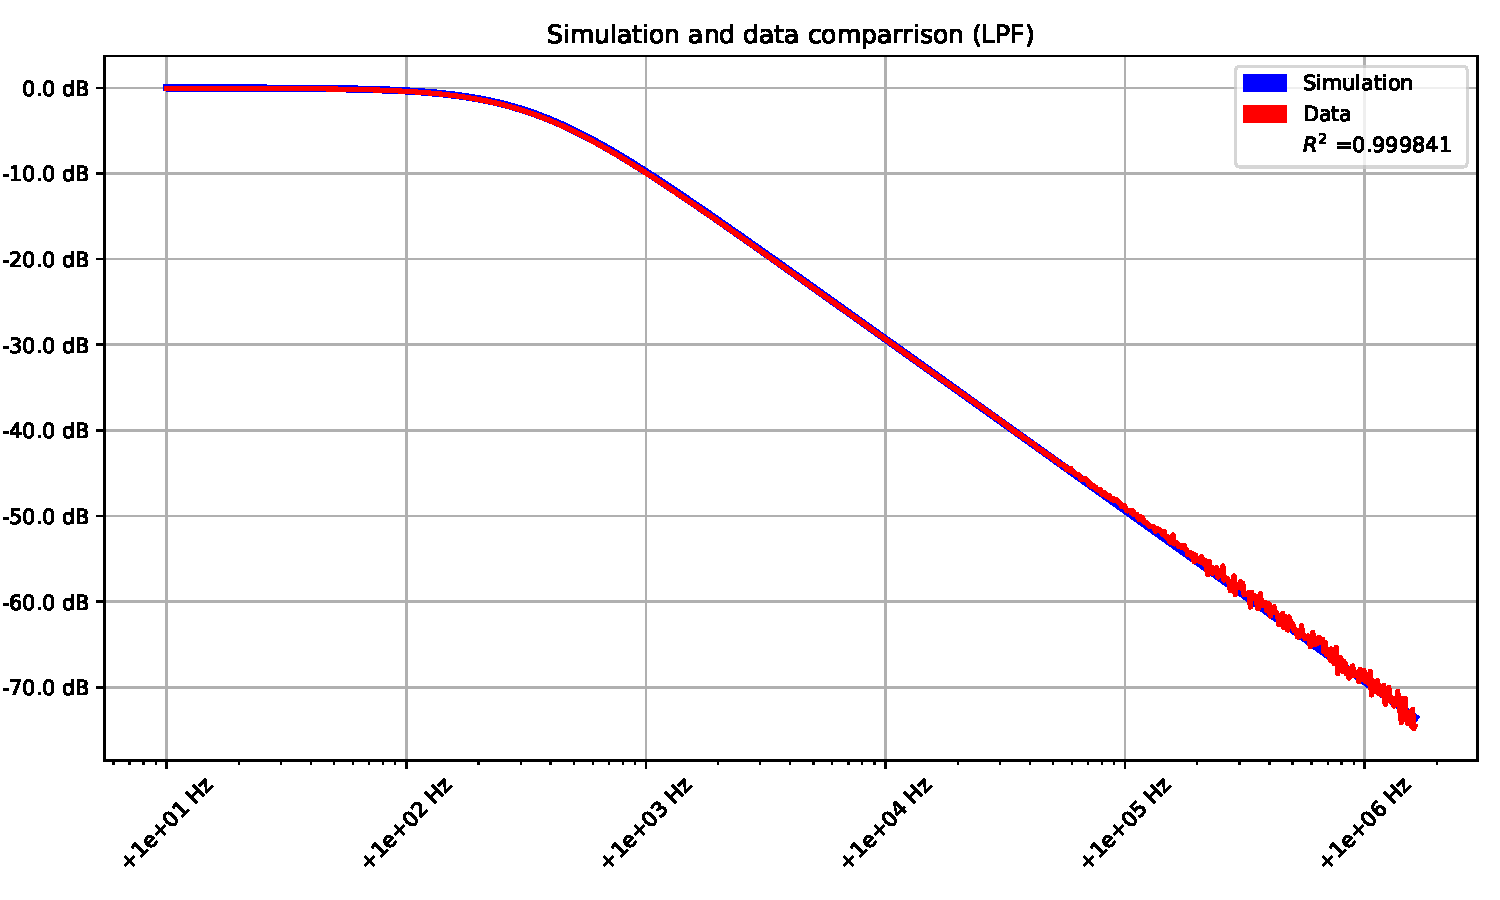
\includegraphics[scale=0.5]{fig/img/bode_LPF_plot.pdf}
	\caption{Low-pass bode plot}
	\label{lp:bode}
\end{figure}
High-pass: \\
Here is the bode plot:
\begin{figure}[H]
\center
	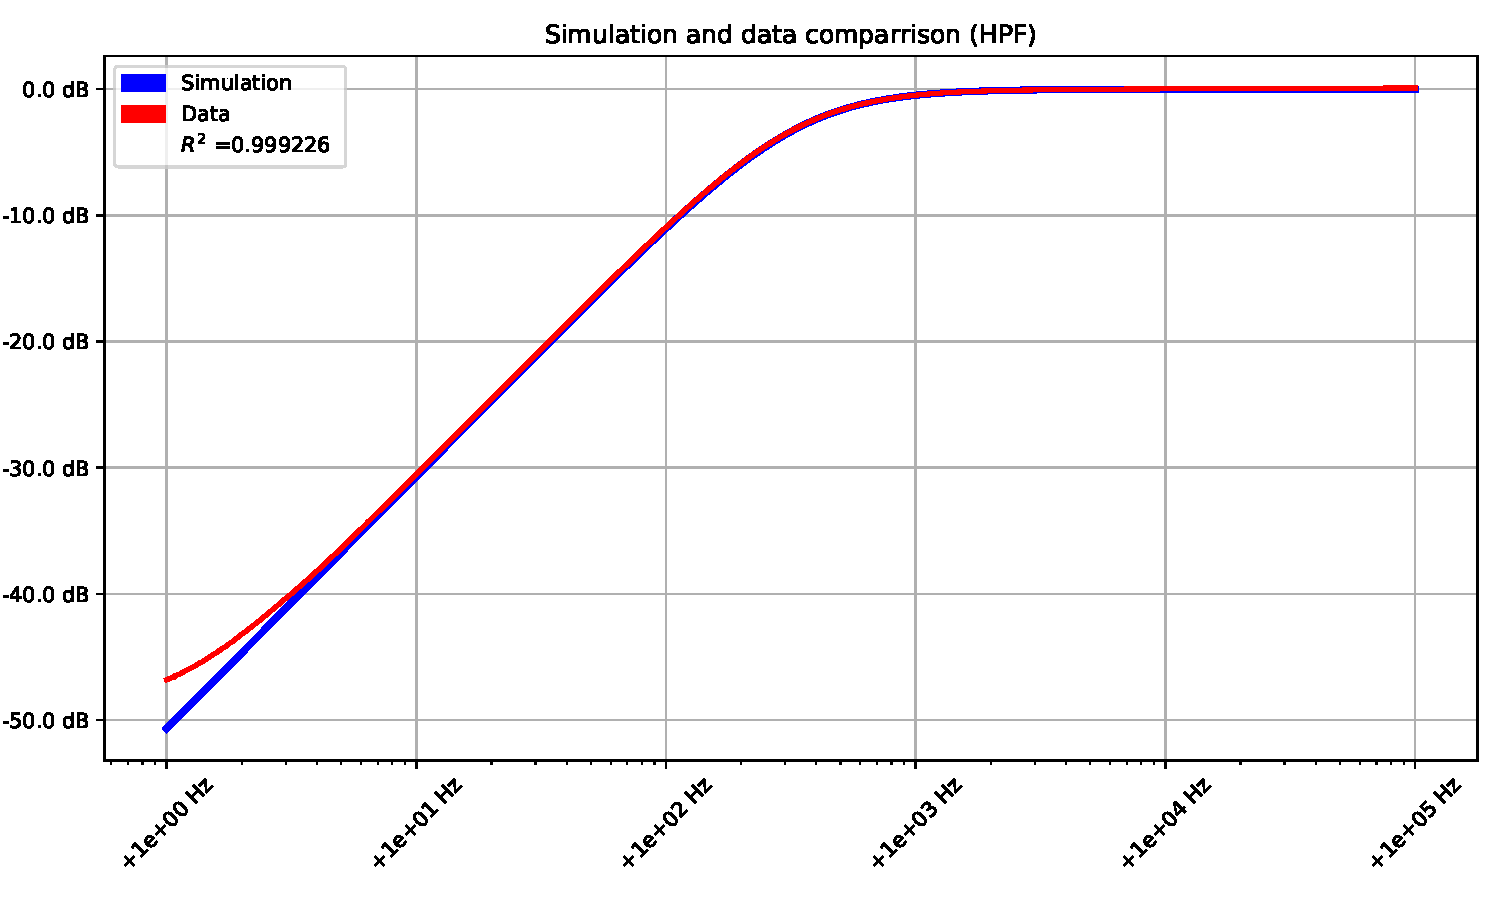
\includegraphics[scale=0.5]{fig/img/bode_HPF_plot.pdf}
	\caption{High-pass bode plot}
	\label{hp:bode}
\end{figure}
\subsection{Comparison}
- Compare the bode plots --> first low then high \\
- Describe source errors (fejlkilder) 